\documentclass[8pt, DIV15, twocolumn]{scrartcl}
\usepackage[utf8]{inputenc}
\usepackage[T1]{fontenc}
\usepackage{amsfonts}
\usepackage[german]{babel}
\usepackage{amsmath}
\usepackage{caption}
\usepackage{float} 
\usepackage{color}
\usepackage{bm}
\usepackage{listings}

\usepackage{graphicx}

\usepackage{ae}
\subject{\vspace{-1\baselineskip}}

\title{Chapter 7 - Lineare Programme}
\date{}

\publishers{\vspace{-.5\baselineskip}}

\begin{document}
\setlength{\abovedisplayskip}{0pt}
\setlength{\belowdisplayskip}{0pt}
\setlength{\parskip}{0pt}
\setlength{\topmargin}{0pt}

 
\maketitle

\thispagestyle{empty}


\section*{Lineares Programm}
Lineare Ungleichung:
\begin{equation*}
y := \mathbf{u}^t \mathbf{x} + u \geq 0
\end{equation*} 

Ungleichungssystem mit l linearen Ungleichungen

\begin{equation*}
y_i := \mathbf{a}_i^t \mathbf{x} + a_i \geq 0
\end{equation*} 
bilden konvexes Polyeder S, \emph{Simplex!}

\subsection*{Def.}
lineare Zielfunktion $z := \mathbf{z}^t \mathbf{x}$.

Lineares Programm:

\begin{equation*}
\begin{aligned}
z &:= \mathbf{z}^t \mathbf{x} &= max! \\
\mathbf{y} &:= A \mathbf{x} + \mathbf{a} &\geq 0
\end{aligned}
\end{equation*} 

Schematische Normalform:

\begin{figure}[ht]
	\centering
  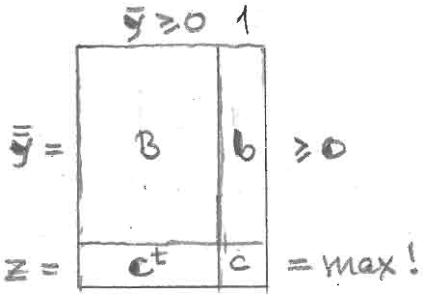
\includegraphics[width=0.2\textwidth]{schematischeNormalform.png}
\end{figure}

\subsection*{Eckentausch}
\begin{figure}[ht]
	\centering
  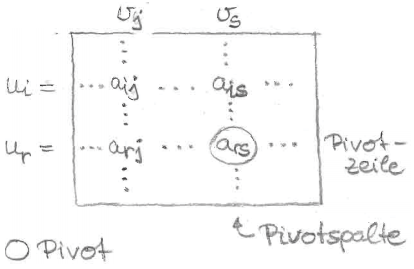
\includegraphics[width=0.2\textwidth]{eckentausch.png}
\end{figure}

AUSTAUSCH:

\begin{lstlisting}[mathescape=true]
Eingabe:
	A = [$a_{ij}$]$_{i,j=1,1}^{m,n}$
	r, s
Ausgabe:
	A' = [$a'_{ij}$]$_{i,j=1,1}^{m,n}$

For i $\neq$ r, j $\neq$ s
	$a'_{ij}$ $\leftarrow$ $a_{ij}$ - $\frac{a_{is} a_{rj}}{a_{rs}}$
For i = r, j $\neq$ s (Pivotzeile)
	$a'_{ij}$ $\leftarrow$ -$\frac{a_{ij}}{a_{rs}}$
For i $\neq$ r, j = s (Pivotspalte)
	$a'_{ij}$ $\leftarrow$ $\frac{a_{ij}}{a_{rs}}$
For i = r, j = s (Pivot)
	$a'_{ij}$ $\leftarrow$ $\frac{i}{a_{rs}}$
\end{lstlisting}

\subsection*{Simplex}
Algorithmus:

\begin{lstlisting}[mathescape=true]
Eingabe:
	Normalform B eines lin. Programms
Ausgabe:
	Normalform geaendert, sodass z($\mathbf{0}$)=c=max

solange ein $c_s$ > 0
	falls alle $b_{is} \geq$ 0
		keine Loesung - Ende
	sonst
		bestimme r so, documentclass
		$\frac{b_r}{b_{rs}} = \max_{b_{is}<0} \frac{b_i}{b_{is}}$
	B $\leftarrow$ AUSTAUSCH(B, r, s)
\end{lstlisting}

Aufwand im worst-case $\Omega \left( m^{\frac{n}{2}} \right)$. In Praxis meist in $O \left( m^2 n \right)$.


\section*{Berechnung der Normalform}
Gegeben ein lineares Programm

\begin{itemize}
	\item finde zulässigen Punkt
	\item mache Punkt zum Ursprung
	\item führe n Tauschs $x_r$ mit $y_r$ durch
\end{itemize}

Damit Ursprung beim Tausch von $x_r$ mit $y_r$ gültig bleibt muss für alle $i > r$ gelten:

\begin{equation*}
a_i - \frac{a_{ir} a_r}{a_{rr}} \geq 0
\end{equation*}

\section*{Duale lineare Programme}
Das lineare Programm 

\begin{equation*}
\begin{aligned}
\mathbf{y} &\geq 0 \\
B^t \mathbf{y} + \mathbf{c} &\leq 0 \\
\mathbf{b}^t \mathbf{y} + c &= min!
\end{aligned}
\end{equation*}

ist dual zu

\begin{equation*}
\begin{aligned}
\mathbf{x} &\geq 0 \\
B \mathbf{x} + \mathbf{b} &\leq 0 \\
\mathbf{c}^t \mathbf{x} + c &= max!
\end{aligned}
\end{equation*}

Ersteres kann transformiert werden zu

\begin{equation*}
\begin{aligned}
\mathbf{y} &\geq 0 \\
-B^t \mathbf{y} - \mathbf{c} &\geq 0 \\
-\mathbf{b}^t \mathbf{y} - c &= max!
\end{aligned}
\end{equation*}

\section*{Ausgleichen mit Maximumsnorm}
$A\mathbf{x} = \mathbf{a}$ überbestimmtes LGS. $\forall \mathbf{x}$ ist das Residuum

\begin{equation*}
\mathbf{r} := \left(r_1 ... r_n \right)^t := A \mathbf{x} - \mathbf{a} \neq 0
\end{equation*}

Wir definieren $x_0 := \frac{1}{r}$ und $\bar{\mathbf{x}} := \mathbf{x} x_0$. Führt zu linearem Programm:

\begin{equation*}
\begin{aligned}
-A\bar{\mathbf{x}} + \mathbf{a} x_0 + \mathbf{e} &\geq 0 \\
A\bar{\mathbf{x}} - \mathbf{a} x_0 + \mathbf{e} &\geq 0 \\
x_0 &= max!
\end{aligned}
\end{equation*}

\end{document}